\documentclass{article}

\usepackage[utf8]{inputenc}
\usepackage[main=english]{babel}

%% These macros specify information about the presentation
\title{ Proyecto de Machine Learning\\ \textbf{ Detección de Digitos en las Manos}}
\author{Carlos Cortés}

%% These additional packages are used within the document:
\usepackage{ragged2e}  % `\justifying` text
\usepackage{booktabs}  % Tables
\usepackage{tabularx}
\usepackage{tikz}      % Diagrams


\usepackage{amsmath, amssymb}
\usepackage{url}       % `\url`s
\usepackage{listings}  % Code listings

\frenchspacing


\begin{document}
  \maketitle
 
    \section{Objetivo}
      Clasificar imágenes de manos haciendo las señas de los dígitos del lenguaje de señas y reconocer el dígito que están haciendo.
      
    \section{Dataset}
        La base de datos de imágenes fue tomada del github de la referencia.\\
        Consta de 2062 imágenes etiquetadas del 0-9~\cite{git}.\\
        Cada imagen es de 100x100 y en formato Jpg (cada entrada es una triada con los valores RGB) por lo que fue necesario convertirlas a escala de grises.\vspace{3mm} \\
        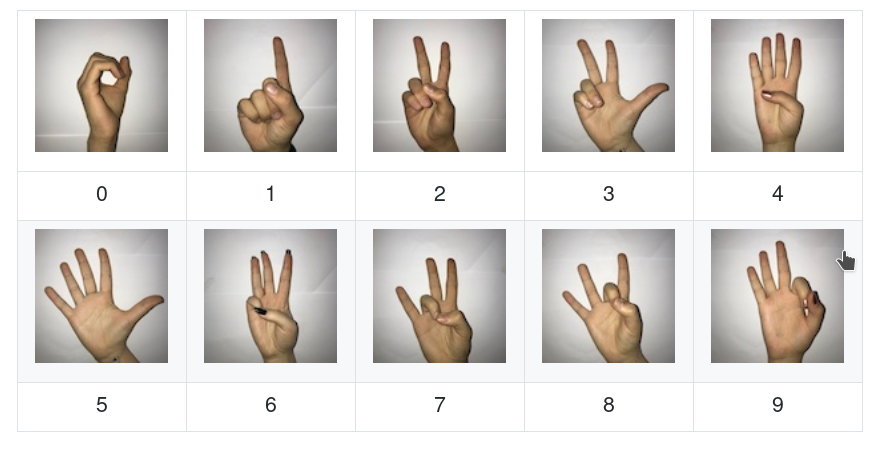
\includegraphics[scale=0.46]{dataset_preview}
    \section{Método}
    
    Lo primordial es recordar que las imágenes son matrices con cada entrada siendo el valor del pixel.\\
    Por lo que se puede desdoblar la matriz en un gran vector para aplicarle algoritmos de machine learning con cada imagen como vector instancia.\\
    Se probó con dos métodos:\\
    \textbf{K-NN: } Es muy sencillo de realizar y da buenos resultados.\\
    \textbf{Regresión Logística: } Supuestamente da mejores resultados.

    
    \section{Implementación}
    La Implementación de los algoritmos fue realizada en C++ para obtener mayor velocidad en la clasificación y utilizando bibliotecas con funciones de aprendizaje automático.
    \subsection{Dependencias}
    \begin{itemize}
    \item \emph{Mlpack}.\\
    Biblioteca principal para métodos de Machine Learning.
    \item \emph{Armadillo}.\\
    Biblioteca para matrices que Mlpack utiliza.
    \item \emph{OpenCV}.\\
    Biblioteca que utilizo para manipular imágenes y convertirlas en vectores.
    \end{itemize}
    
    \subsection{Breve Descripción del Programa}
    El programa tiene 4 funciones principales:
    \begin{itemize}
     \item \textbf{Actualizar la Base de datos.} Lee todas las imágenes de la carpeta \emph{Dataset}, las convierte en una matriz y escribe un archivo \texttt{.csv}  con los datos y otro con las 
clases.
    \item \textbf{Modo Interactivo.} Inicia un \emph{prompt} en el que puedes indicarle la ruta de la imagen a clasificar.
    \item \textbf{Test.} Parte el Dataset en conjunto de entrenamiento y de prueba y luego estima el poder predictivo.
    \item \textbf{Cámara.} Toma como input a clasificar la imagen de la cámara.
    \end{itemize}
   
    \section{Mejor Puntaje}
    \textbf{El mejor puntaje obtenido por el clasificador}\\
    Partiendo el Dataset en 1856 de entramiento y 206 de prueba.\\
    Con k = 10 vecinos más cercanos.\\
    \subsection{K-NN}
        154 casos correctos.\\
        Porcentaje = $74.75\%$.\\
        Entre ($68.85\%$ , $80.65\%$) al $95\%$ de confianza.
    \subsection{Regresión Logística}
        25 casos correctos.\\
        Porcentaje = $12.13\%$.\\
        Entre ($7.69\%$ , $16.57\%$) al $95\%$ de confianza.

      \begin{thebibliography}{9}
        \bibitem{git}
            ardamavi.
            Sign-Language-Digits-Dataset.
            2018.
            Recuperado de \url{https://github.com/ardamavi/Sign-Language-Digits-Dataset}
      \end{thebibliography}
\end{document}
